\subsection{Giao diện cấu hình khảo sát}

\begin{figure}[H]
    \centering
    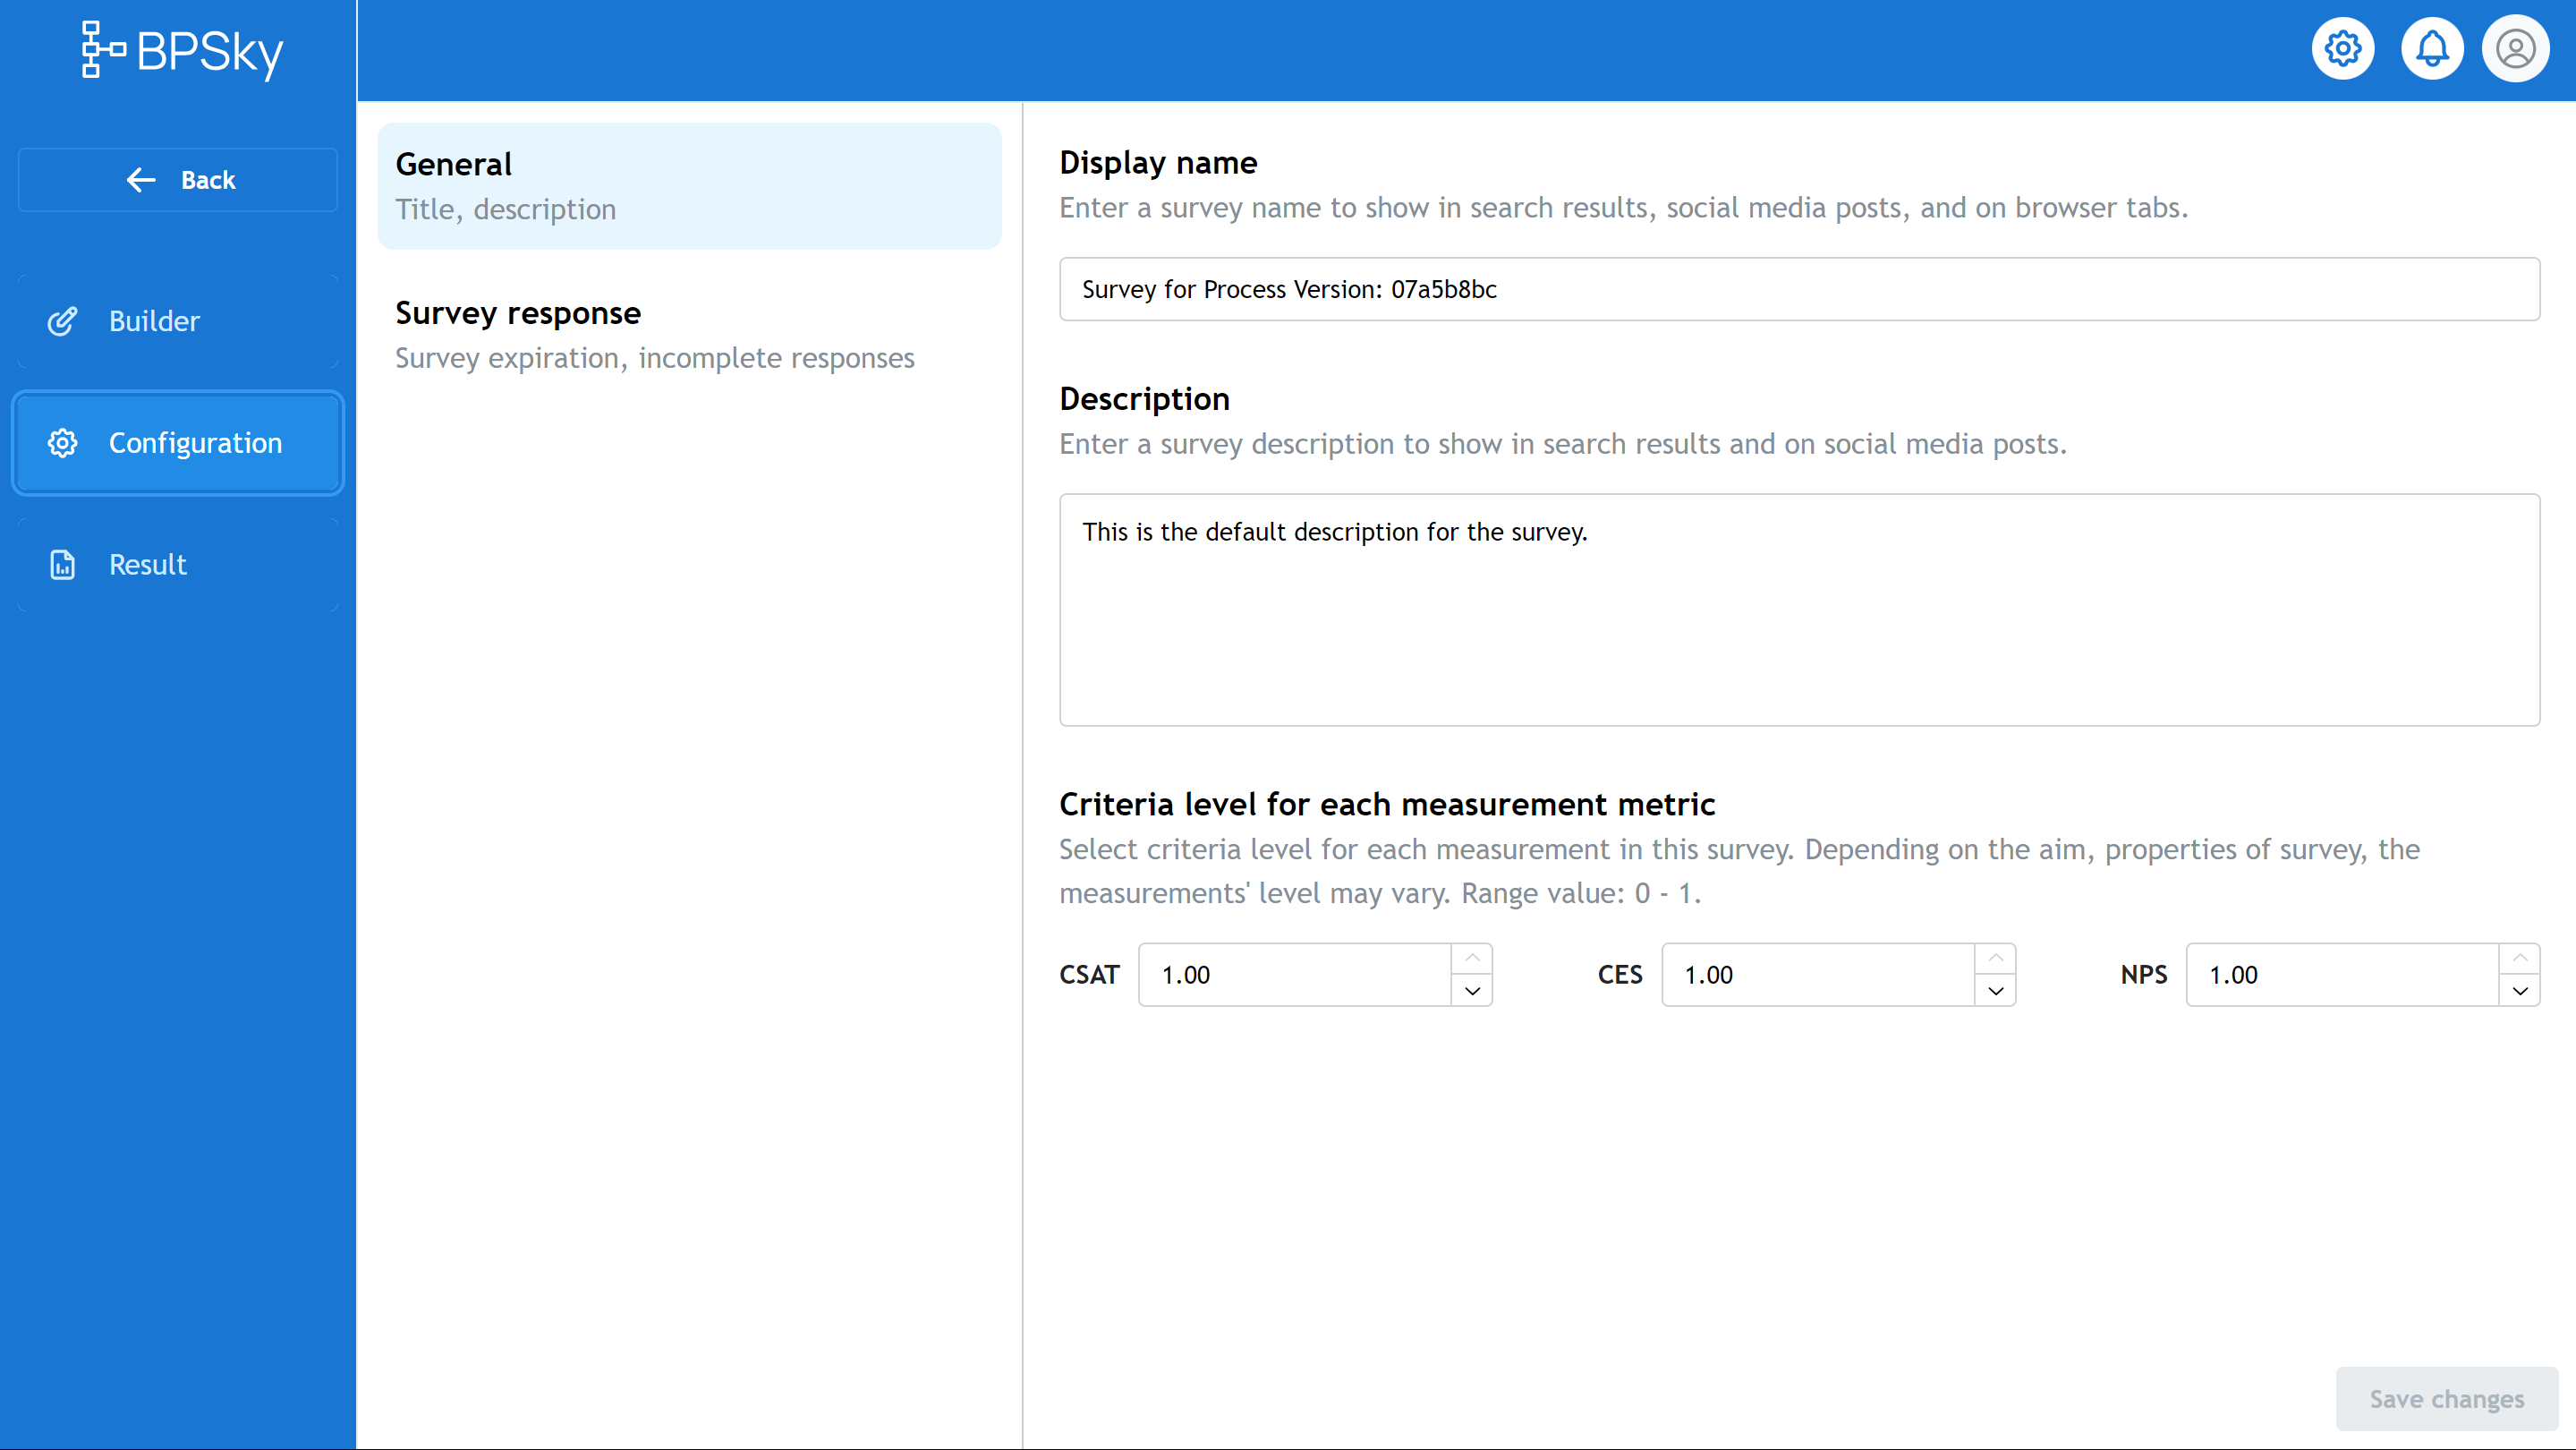
\includegraphics[ width = 0.8\linewidth]{Content/Hiện thực hệ thống/documents/Hiện thực giao diện người dùng/images/SurveyGeneralConfiguration.png}
    \vspace{0.5cm}
    \caption{Giao diện cấu hình thông tin chung của bảng khảo sát}
    \label{fig: Giao diện cấu hình thông tin chung của bảng khảo sát}
\end{figure}

Người dùng sau khi chọn Configuration trên thanh điều hướng thì hệ thống sẽ chuyển hướng người dùng tới giao diện cấu hình thông tin chung của bảng khảo sát. Tại đây, người dùng có thể thay đổi các cấu hình liên quan tới bảng khảo sát như tên, mô tả và các trọng số của các loại câu hỏi trong bảng khảo sát. Các cấu hình này sẽ ảnh hưởng đến việc hiển thị và tính toán kết quả của bảng khảo sát.

\begin{figure}[H]
    \centering
    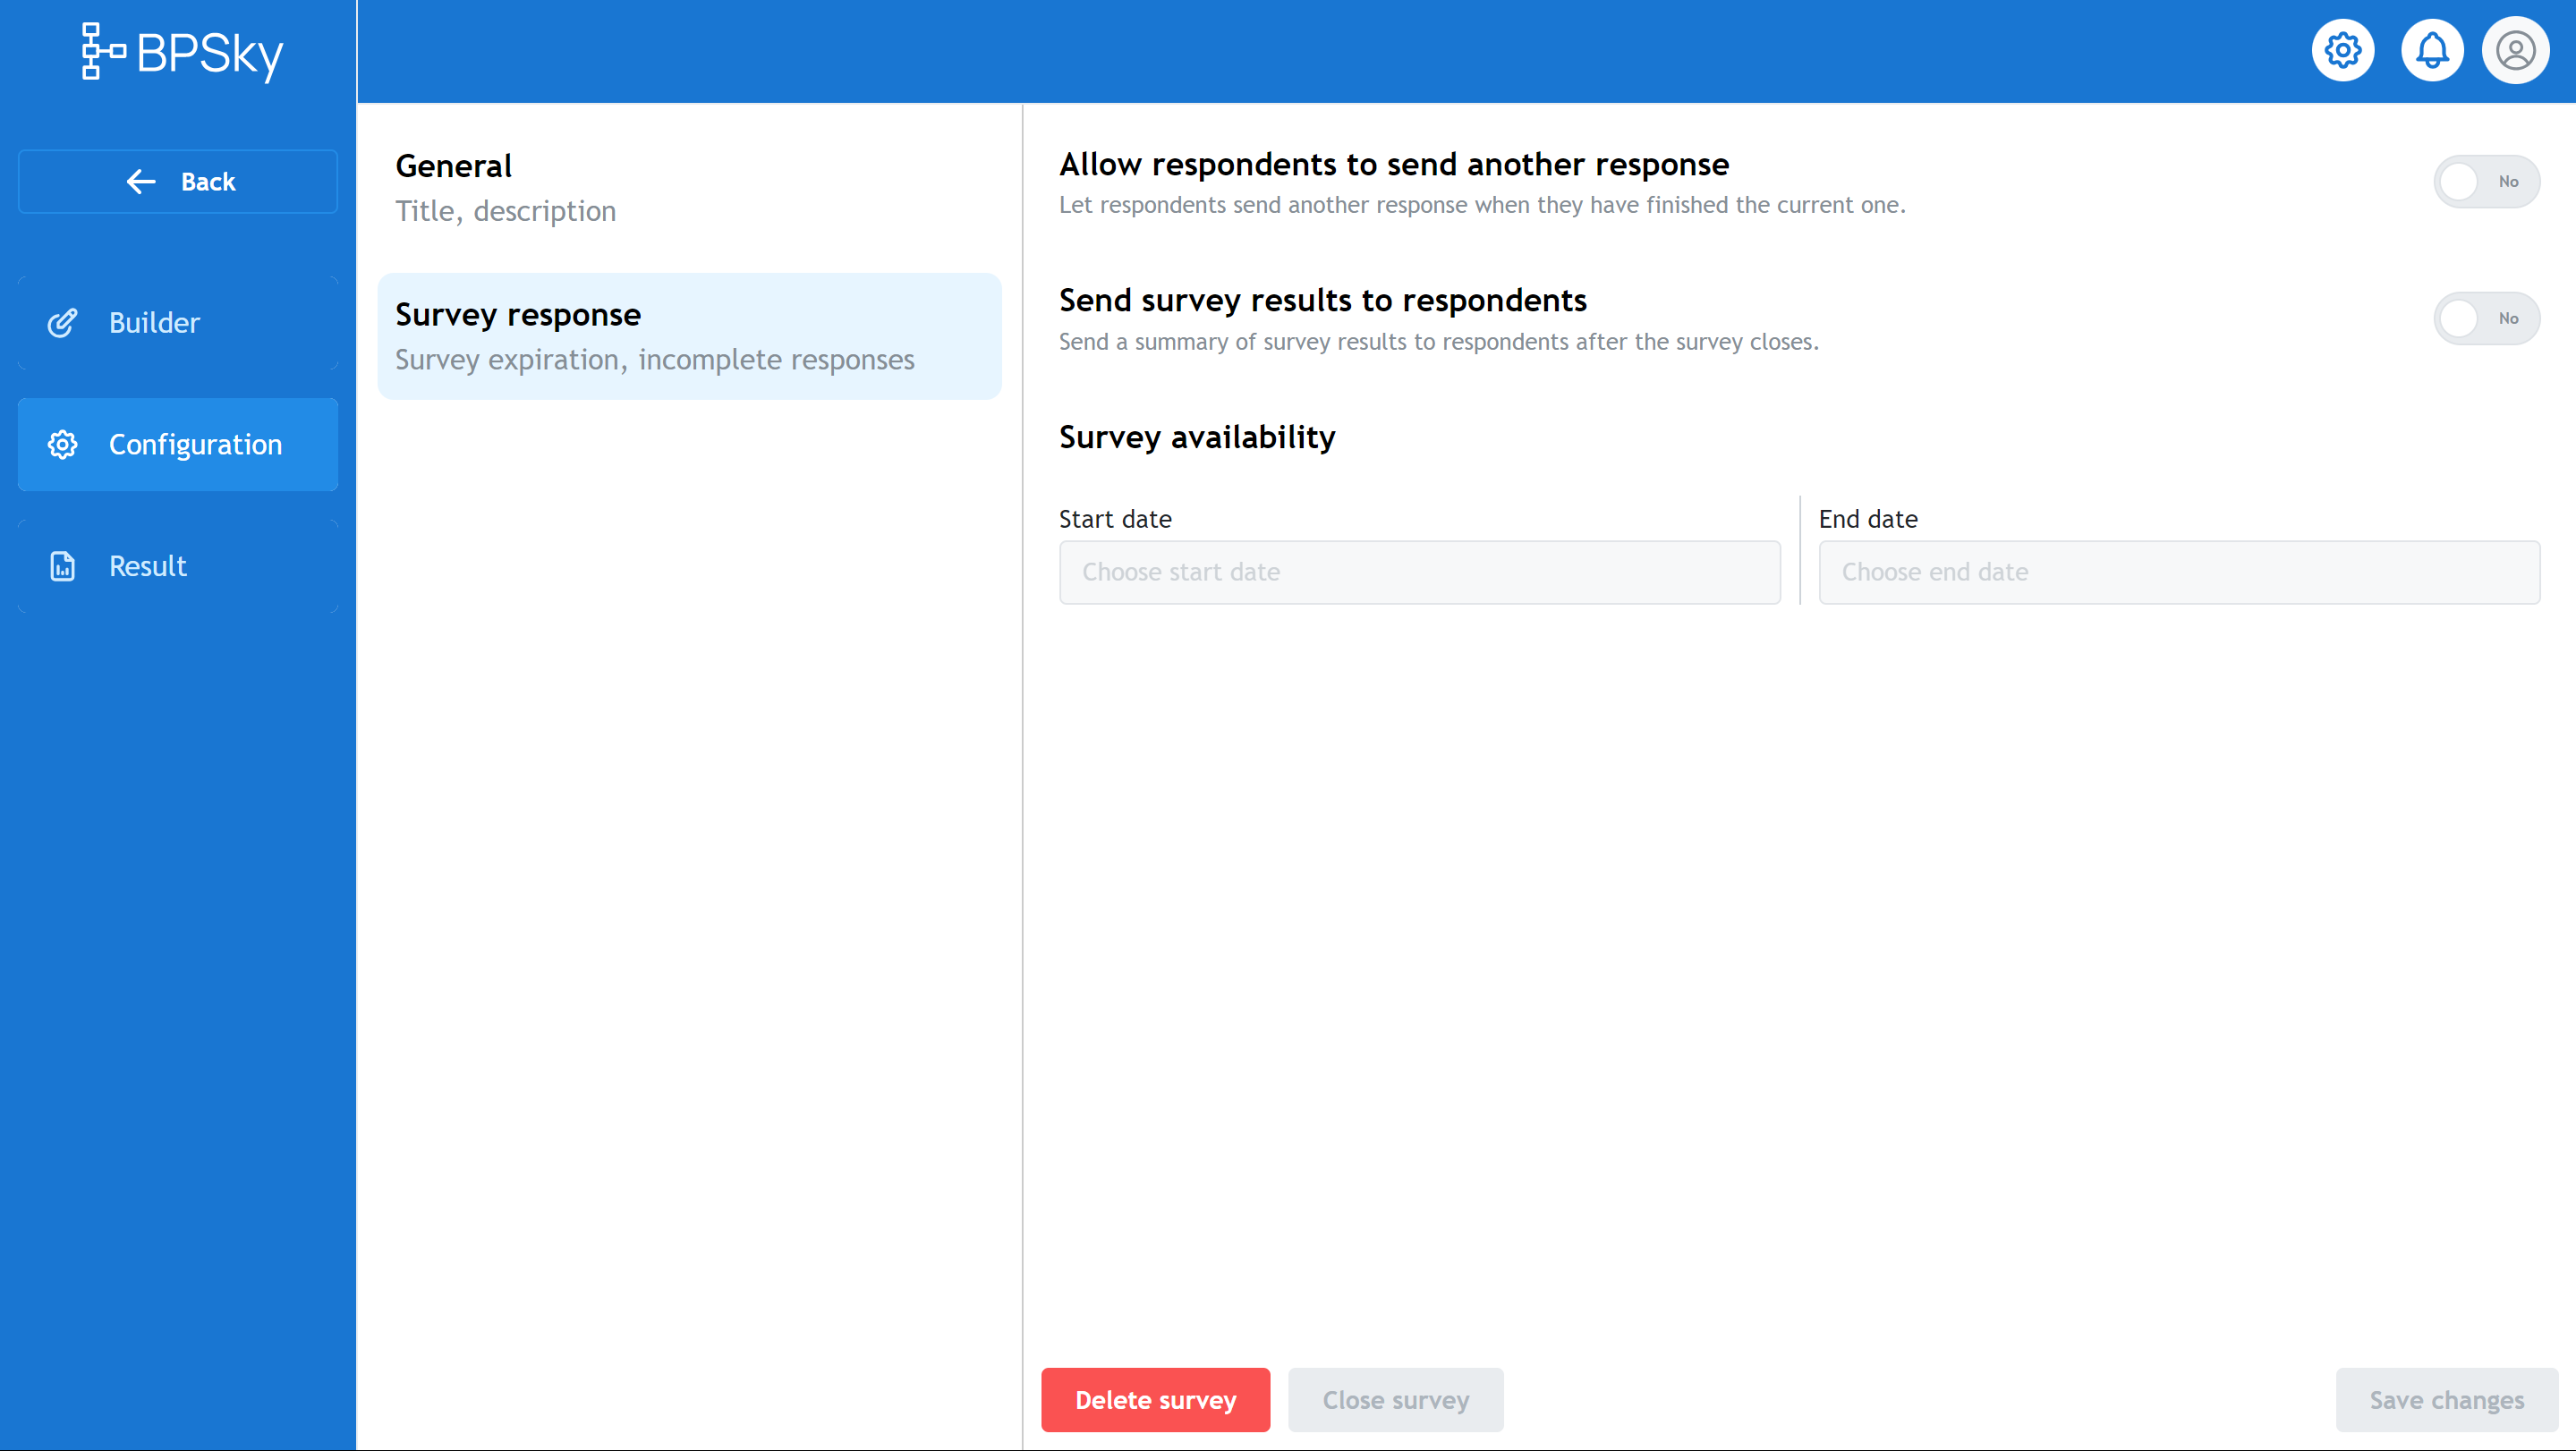
\includegraphics[ width = 0.8\linewidth]{Content/Hiện thực hệ thống/documents/Hiện thực giao diện người dùng/images/SurveyResponseConfiguration.png}
    \vspace{0.5cm}
    \caption{Giao diện cấu hình phản hồi của bảng khảo sát}
    \label{fig: Giao diện cấu hình phản hồi của bảng khảo sát}
\end{figure}

Ngoài ra, người dùng có thể chọn mục Survey response để chuyển hướng tới giao diện cấu hình phản hồi của bảng khảo sát. Tại đây, người dùng có thể cấu hình các thông tin liên quan tới phản hồi của bảng khảo sát như thông kết quả sau khi khảo sát hoàn thành qua hòm thư, cho phép người dùng thực hiện một/nhiều lần khảo sát và thời gian đóng/mở khảo sát.